
\documentclass[12pt, a4paper]{article}

% including packages
\usepackage[utf8]{inputenc}
\usepackage{amsmath}
\usepackage{graphicx}
\usepackage{wrapfig}

\graphicspath{ {images/} }

% title
\title{Using Genetic Algorithms to Find Approximations for the Minimum Vertex Cover Problem}
\author{}
\date{}




% document begins here
\begin{document}

{
\begin{wrapfigure}{r}{0.25\textwidth}
\hfill
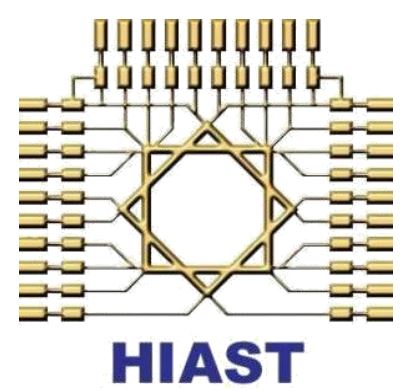
\includegraphics[width=0.9\linewidth]{hiast}
\end{wrapfigure}

\setlength{\parindent}{0cm}
Syrian Arab Republic\\
Higher Institute for Applied Sciences and Technology\\
Informatics Department\\
Fourth Year\\
}

%\begin{flushleft}
\noindent Syrian Arab Republic\\
Higher Institute for Applied Sciences and Technology\\
Informatics Department \\
Fourth Year\\
%\end{flushleft}



{\let\newpage\relax\maketitle}

\begin{center}
\begin{align*}
\text{Author: }					& \textit{Farouk Hjabo} \\
\text{Academic Supervisor: }	& \textit{Dr. Said Desouki} \\
\text{General Supervisor: }		& \textit{Dr. Kadan Aljoumaa} \\
\text{Langauge Supervisor: }	& \textit{Mr. Fahmi Alammareen} \\
\end{align*}
\end{center}

\vfill
\centerline{\date{\today}}
\pagebreak

\section{intro}
hislhdf
\subsection{intro-sub}
dfsfafs

\section{conc}
lsdjfslfd
\end{document}
